\topsection[sec:impl]{Implementation}

This section is the first half of phase~4: what was built and in which environment it was tested. The
experiments follow in Section~\ref{sec:eval}.

\subsection{Code organisation}
One core library holds all the security logic. The command line, the REST API, the machine-learning pipeline,
the deployment gateway, the attack scenarios and the CI workflows call that same library, so there is exactly
one implementation of hashing, signing and verification (Figure~\ref{fig:system}). The dashboard uses only the
HTTP API. Table~\ref{tab:code} gives the size of each component.

\begin{figure}[!htb]
\centering
\begin{tikzpicture}[x=1cm,y=1cm,font=\sffamily\fontsize{7.7}{9.6}\selectfont,
  box/.style={draw=cgnavy,line width=0.6pt,rounded corners=2.5pt,align=center,fill=white,minimum height=0.86cm,inner sep=2pt},
  grp/.style={rounded corners=3pt,fill=cgband,inner sep=0pt},
  lab/.style={font=\sffamily\bfseries\fontsize{8}{10}\selectfont,text=cgnavy,anchor=north west},
  arr/.style={-{Latex[length=1.9mm,width=1.5mm]},line width=0.7pt,color=cgteal}]
% consumers
\node[grp,minimum width=15cm,minimum height=1.62cm] (g1) at (7.5,0) {};
\node[lab] at (0.15,0.76) {Consumers};
\foreach \x/\t in {1.62/{Command line\\\code{cli/}},4.56/{ML pipeline\\\code{ml\_pipeline/}},7.5/{Attack scenarios\\\code{attacks/}},10.44/{CI workflows\\\code{.github/}},13.38/{Dashboard\\\code{dashboard/}}}{
  \node[box,minimum width=2.72cm] at (\x,-0.2) {\t};
}
% API + gateway
\node[box,minimum width=4.2cm,fill=white] (api) at (11.9,-1.9) {REST API (FastAPI)\enskip\code{api/}};
\node[box,minimum width=4.2cm,fill=white] (gw) at (5.0,-1.9) {Deployment gateway\enskip\code{deployment/}};
% core
\node[grp,minimum width=15cm,minimum height=2.5cm] (g2) at (7.5,-4.15) {};
\node[lab] at (0.15,-2.98) {Core library\enskip\code{chainguard/}};
\foreach \x/\t in {1.3/{Hashing\\SHA-256},3.78/{Canonical JSON\\Ed25519 signing},6.26/{Manifests\\Merkle trees},8.74/{Policy\\content checks},11.22/{Verifier\\V0 to V9},13.7/{Registry\\trust log}}{
  \node[box,minimum width=2.38cm] at (\x,-3.95) {\t};
}
\node[font=\sffamily\fontsize{7.3}{9}\selectfont,text=cgmuted,anchor=west] at (0.15,-4.95) {External models, in-toto, DSSE and SLSA export, verified file reads};
% storage
\node[grp,minimum width=15cm,minimum height=1.5cm] (g3) at (7.5,-6.5) {};
\node[lab] at (0.15,-5.83) {Workspace};
\foreach \x/\t in {1.95/{Signed manifests (source of truth)},5.65/{Data and model files},9.35/{SQLite index (untrusted)},13.05/{Keys and pin (trusted)}}{
  \node[box,minimum width=3.55cm,minimum height=0.62cm,font=\sffamily\fontsize{7.2}{9}\selectfont] at (\x,-6.72) {\t};
}
\draw[arr] (13.38,-0.63) -- (13.38,-1.47);
\draw[arr] (5.0,-0.81) -- (gw.north);
\draw[arr] (gw.south) -- (5.0,-2.9);
\draw[arr] (api.south) -- (11.9,-2.9);
\draw[arr] (api.west) -- (gw.east);
\draw[arr] (1.62,-0.81) -- (1.62,-2.9);
\draw[arr] (7.5,-5.4) -- (7.5,-5.75);
\end{tikzpicture}
\caption{System architecture. Every consumer goes through the core library; the dashboard goes through the
API. The signed manifests on disk are the source of truth and the SQLite index is a convenience copy.}
\label{fig:system}
\end{figure}

{\tablefont
\begin{xltabular}{\textwidth}{P{3.0cm}P{2.2cm}rrL}
\caption{Size of the implementation at the final commit (Python files and lines, counted with comments and blank lines).}\label{tab:code}\\
\toprule
\headrow\hd{Component} & \hd{Folder} & \hd{Files} & \hd{Lines} & \hd{Content} \\
\midrule
\endfirsthead
\toprule
\headrow\hd{Component} & \hd{Folder} & \hd{Files} & \hd{Lines} & \hd{Content} \\
\midrule
\endhead
\bottomrule
\endfoot
Core library & \code{chainguard/} & 32 & 3,592 & Hashing, canonical JSON, signing and keys, manifests, Merkle trees, policy, content checks, verifier, registry, trust log, external models, export \\
Attack scenarios & \code{attacks/} & 10 & 1,158 & Scenarios A to G and their runner \\
Scripts & \code{scripts/} & 10 & 1,578 & Benchmarks, figures, demonstration, validation run, supplementary experiments \\
Dashboard & \code{dashboard/} & 11 & 824 & Streamlit, nine pages \\
REST API & \code{api/} & 11 & 627 & FastAPI, 26 routes \\
ML pipeline & \code{ml\_pipeline/} & 7 & 567 & Dataset export, CNN, training, fine-tuning, evaluation \\
Command line & \code{cli/} & 2 & 319 & Keys, register, verify, revoke, export, import \\
Deployment gateway & \code{deployment/} & 2 & 175 & Stage 4 \\
\midrule
Tests & \code{tests/} & 21 & 1,603 & 168 tests, unit and integration \\
\end{xltabular}}

\subsection{Cryptographic implementation}
\textbf{Hashing.} SHA-256, read in chunks of 1\,MiB so that memory use is constant. SHA-256 is the digest of
OCI images, Sigstore, SLSA and in-toto, which keeps the exports interoperable.

\textbf{Signatures.} Ed25519 through the Python \code{cryptography} library, which uses OpenSSL. Signatures are
64 bytes and public keys 32 bytes. Signing is deterministic, which removes the nonce-reuse failure that has
leaked ECDSA keys in practice. Private keys are PKCS\#8 files with owner-only permissions, or CI secrets passed
in environment variables and never written to disk. The \code{algorithm} field of each signature entry allows a
later migration to a post-quantum scheme.

\textbf{Canonical serialisation.} Signatures are computed over the canonical JSON of the payload: sorted keys,
compact separators, UTF-8. The verifier digests the payload \emph{as read from disk}, not after parsing it into
objects, so even one added field breaks the verification.

\textbf{Merkle trees.} Our own implementation of the RFC~6962 construction, with separate prefixes for leaves
and inner nodes and a split at the largest power of two. One leaf per line of the CSV file.

\textbf{Safe reads.} The function \code{open\_verified()} verifies the chain, reads the file once, hashes those
bytes and returns them. Training and the gateway load data and models from those bytes only. Model weights are
stored as safetensors, and the gateway refuses pickle-based formats.

\subsection{Machine-learning pipeline}
The pipeline uses the digits dataset shipped with scikit-learn: 1,797 images of 8 by 8 pixels, split into 1,000
training, 437 fine-tuning and 360 held-out samples. The model is a small convolutional network with 38,282
parameters. The base model is trained for 15 epochs and fine-tuned for 8, with the seed 42. On the reference
run the deployed model reaches a clean test accuracy of 95.0\,\%. The model is small on purpose: the
cryptographic mechanisms do not depend on its size, and a full run that trains real models takes seconds, so
every experiment is reproducible on a laptop.

Before a dataset is signed, three content checks run on it (Table~\ref{tab:semantic}). Their results are
written into the signed manifest. A flag never blocks the signature: it travels with the artifact and becomes
check V9 at verification.

\begin{table}[H]
\caption{The three content checks that run before a dataset is signed.}
\label{tab:semantic}
\tablefont
\begin{tabularx}{\textwidth}{P{3.0cm}P{5.3cm}L}
\toprule
\headrow\hd{Check} & \hd{Detects} & \hd{Known blind spot} \\
\midrule
Label distribution & Heavy label flipping or poisoning aimed at one class (chi-square test against a reference) & Low poisoning rates \\
Duplicate rows & Amplification by duplication (more than 2\,\% of duplicates) & Near-duplicates \\
Corner trigger & A saturated 2 by 2 patch in a corner, the BadNets trigger & Any other trigger shape (variant E4) \\
\bottomrule
\end{tabularx}
\end{table}

\subsection{Interfaces}
\textbf{Command line.} \code{python -m cli.main} creates the role keys, registers and signs an artifact,
verifies it (exit code 0 for \st{VERIFIED}, 2 for \st{WARNING}, 1 for \st{FAILED}), revokes an artifact or a
key, prints the trust log, exports an attestation and imports an external model.

\textbf{REST API.} A FastAPI application with 26 routes: read the registry and the provenance graph, register,
verify, deploy through the gateway, revoke, export an attestation, read the trust log, register a publisher and
import an external model, read events and metrics. Interactive documentation is served at \code{/docs}.

\textbf{Dashboard.} A Streamlit application with nine pages: overview, provenance chain
(Figure~\ref{fig:dash}), verification of an artifact, attack lab with live tampering, security events, metrics,
external models, trust log with bypass attempts in a sandbox, and a comparison page.

\begin{figure}[!htb]
\centering
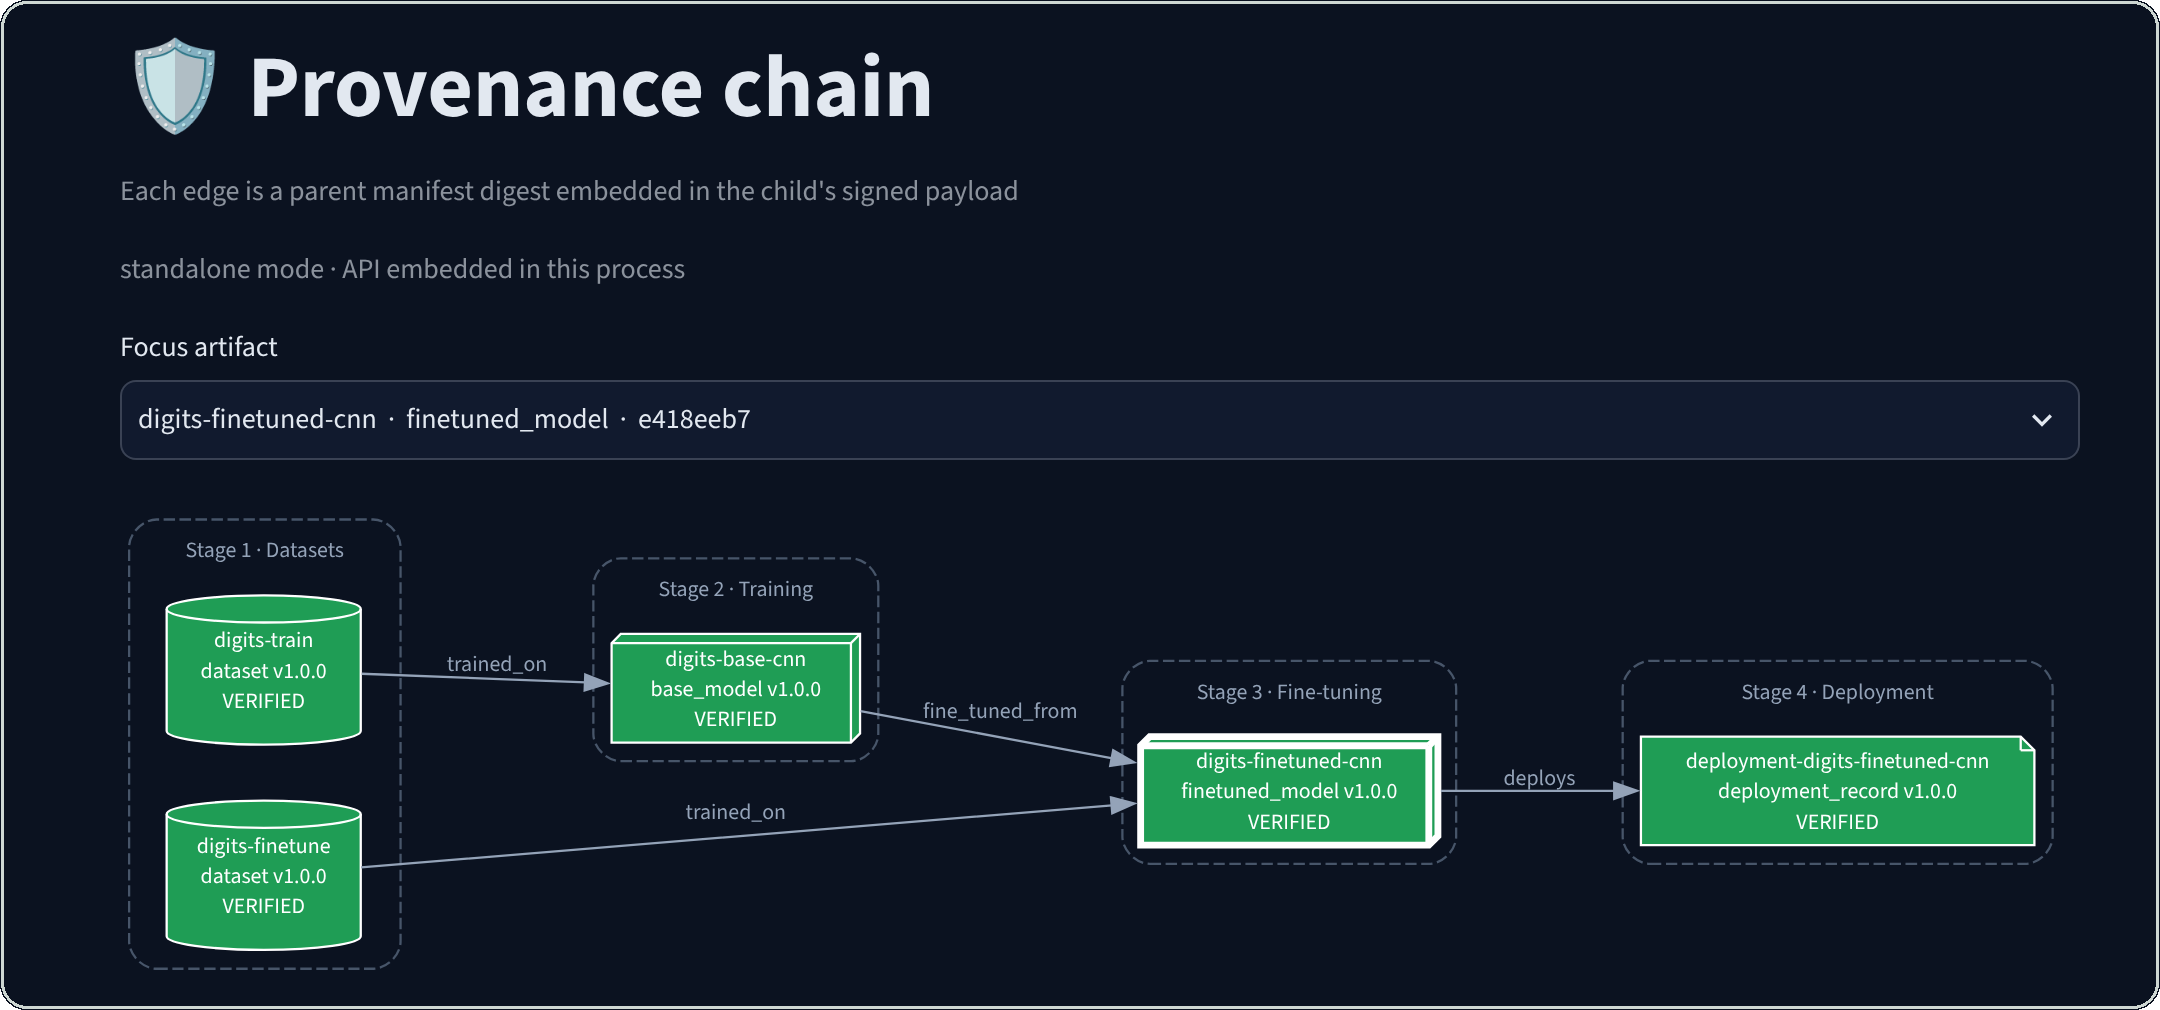
\includegraphics[width=0.86\textwidth]{figures/shot_provenance.png}
\caption{Dashboard, provenance chain page (run of 10~November 2026). Each edge is a parent manifest digest
embedded in the signed payload of the child. The colours show the last verification result stored in the
index; the verifier itself never trusts that stored status.}
\label{fig:dash}
\end{figure}

\subsection{Docker and continuous integration}
A Docker Compose file starts three services on one shared volume: the pipeline, which runs once and exits; the
API on port 8000; and the dashboard on port 8501.

Two GitHub Actions workflows run on every push to the main branch:
\begin{itemize}
\item \code{ci}: the linter, a guard that fails if a private key is committed, and the 168 tests on
  Python~3.11.
\item \code{attest-and-verify}: it creates keys for the run, executes the four-stage attested pipeline and
  fails if the gateway blocks, verifies the deployed model again independently, runs a negative control (one
  flipped byte of the deployed model must give \st{FAILED}), runs the attack scenarios A to D, F and G (43
  variants) and uploads the evidence. An optional job signs with Sigstore; it is disabled by default.
\end{itemize}
This workflow is the automated attestation in CI/CD that the brief suggests: a release is refused unless the
gateway returns \st{VERIFIED}.

\subsection{Test environments}
{\tablefont
\begin{xltabular}{\textwidth}{P{4.9cm}LP{2.3cm}}
\caption{Where the system was executed.}\label{tab:env}\\
\toprule
\headrow\hd{Environment} & \hd{What ran there} & \hd{Date (2026)} \\
\midrule
\endfirsthead
\toprule
\headrow\hd{Environment} & \hd{What ran there} & \hd{Date (2026)} \\
\midrule
\endhead
\bottomrule
\endfoot
Reference environment: cloud Linux container, Intel Xeon at 2.10\,GHz with two logical cores, 8.2\,GB of memory, no GPU, Python 3.13.16, PyTorch 2.15.0 on CPU & The full validation run: linter, 168 tests, pipeline, the 48 variants, every benchmark and figure. Supplementary experiments & 9~November; supplementary runs on 10~November \\
GitHub-hosted runner (Ubuntu, Python 3.11.18, PyTorch 2.15.0) & Both workflows on every push: 168 tests, attested pipeline, negative control, 43 attack variants & 9 and 10~November \\
Team laptop (MacBook Air), Docker & Image build and Compose stack: the four-stage pipeline (\st{VERIFIED}, deployed, clean accuracy 95.0\,\%), the API health check and the dashboard & 16~October \\
Any reader's browser, on the website & Checks V1 and V3 on the deployed model of experiment E2, and the model itself & since 10~November \\
\end{xltabular}}

The benchmarks of Section~\ref{sec:eval} were measured in the reference environment only. Shared CI runners are
not a stable timing environment, and the full test and benchmark run has not been repeated on team hardware.

\subsection{Technologies of the brief}
Python and PyTorch are used throughout. For signing, the brief offers Sigstore, cosign or custom signing with
OpenSSL: we use custom Ed25519 signing on the OpenSSL backend of the \code{cryptography} library, with the
optional Sigstore job in CI. The Merkle tree is our own implementation of RFC~6962. Docker and GitHub Actions
are used as described above. Hyperledger Fabric and blockchain anchoring, both optional, are not used; the
signed trust log takes their place (Section~\ref{sec:trustlog}).
